\subsection{Tabellen über mehrere Seiten}

\begin{frame}[fragile]
\frametitle{Tabellen über mehrere Seiten}
\framesubtitle{Das Paket \pkg{longtable}}
\begin{itemize}
\item Tabellen mit Seitenumbruch mit dem Paket \pkg{longtable} erzeugen.\pause
\item Syntax genau wie bei einer normalen Tabelle. \pause
\item Aufruf über die \umg{longtable}-Umgebung. \pause
\item Nachteil: Kann nicht in \umg{table}-Umgebung genutzt werden, da sonst nicht am Ende umgebrochen wird.\pause
\item Arbeit mit der \umg{minipage}-Umgebung: Diese kann innerhalb einer \umg{longtable} auch über mehrere Seiten laufen. 
\end{itemize}
\end{frame}

\begin{frame}[fragile]
\frametitle{Tabellen über mehrere Seiten: Ein Beispiel}
\footnotesize
\begin{codeblock}
% benutze das paket fancyvrb
\begin{Verbatim}[fontsize=\tiny]  
\begin{longtable}{|c|c|}
\hline Zeit $t$ & Geschwindigkeit $v_{\text{B}}$  \\ \hline 
\endfirsthead

\multicolumn{2}{c}{Hier gehts weiter...} \\ \hline 
Zeit t & Geschwindigkeit $v_{\text{B}}$  \\ \hline 
\endhead

\hline \multicolumn{2}{|r|}{{Weiter auf der nächsten Seite}} \\ 
\hline
\endfoot

\hline \hline
\endlastfoot

1 & 2 \\ 
 ...
\end{longtable}
\end{Verbatim}
\end{codeblock}
\end{frame}

\begin{frame}[fragile]
\frametitle{Tabellen über mehrere Seiten: Ein Beispiel}
\begin{figure}
 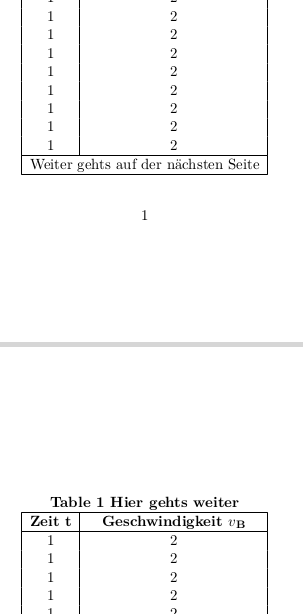
\includegraphics[height=0.8\textheight]{images/longtable_v2.png}
\end{figure}

\end{frame}

\begin{frame}[fragile]
\frametitle{Tabellen über mehrere Seiten}
\framesubtitle{Wichtiges}
\begin{itemize}
\item mit \cmd{endfirsthead} definiert man die oberste Zeile der Tabelle 
\item mit \cmd{endhead} definiert man die oberste Zeile der Tabelle auf den folgenden Seiten
\item mit \cmd{endfoot} und \cmd{endlastfoot} analog die letzten Zeilen
\end{itemize}
\end{frame}

